\documentclass[11pt, a4paper]{article}
\usepackage{amsmath, amssymb, amsthm}
\usepackage{geometry}
\usepackage{hyperref}
\usepackage{xcolor}
\usepackage{tikz}
\usepackage{tikz-cd}
\usepackage{mathtools}
\usepackage{enumitem}
\usepackage{framed}

\geometry{margin=2.5cm}

\usetikzlibrary{arrows.meta, positioning, calc}

% ── Theorem environments ──────────────────────────────────────────────────────
\newtheorem{theorem}{Theorem}[section]
\newtheorem{lemma}[theorem]{Lemma}
\newtheorem{corollary}[theorem]{Corollary}
\newtheorem{definition}[theorem]{Definition}
\newtheorem{example}[theorem]{Example}
\newtheorem{remark}[theorem]{Remark}

% ── Colour palette ────────────────────────────────────────────────────────────
\definecolor{deepblue}{RGB}{30,80,160}
\definecolor{deepred}{RGB}{160,30,50}
\definecolor{deepgreen}{RGB}{20,130,60}
\definecolor{deeporange}{RGB}{200,100,0}
\definecolor{deeppurple}{RGB}{120,40,160}
\definecolor{lightgray}{RGB}{240,240,245}

% ── Named rule environment ────────────────────────────────────────────────────
\newenvironment{rulebox}[1]{%
  \medskip\noindent\textbf{\textcolor{deepblue}{#1}}\nopagebreak\par\noindent%
  \begin{framed}\small%
}{\end{framed}\medskip}

% ── Notation ─────────────────────────────────────────────────────────────────
\newcommand{\III}{\mathbb{I}}
\newcommand{\FFF}{\mathbb{F}}
\newcommand{\UU}{\mathcal{U}}
\newcommand{\pt}[1]{\mathsf{#1}}
\newcommand{\GlueT}{\pt{Glue}}
\newcommand{\glueT}{\pt{glue}}
\newcommand{\unglueT}{\pt{unglue}}
\newcommand{\compT}{\pt{comp}}
\newcommand{\transpT}{\pt{transp}}
\newcommand{\fillT}{\pt{fill}}
\newcommand{\equivT}{\pt{equiv}}
\newcommand{\EquivT}{\pt{Equiv}}
\newcommand{\isContrT}{\pt{isContr}}
\newcommand{\isEquivT}{\pt{isEquiv}}
\newcommand{\contrT}{\pt{contr}}
\newcommand{\pres}[1]{\pt{pres}^{#1}}
\newcommand{\eqop}[1]{\pt{equiv}^{#1}}
\newcommand{\PathT}{\pt{Path}}
\newcommand{\sys}[2]{[#1 \mapsto #2]}
\newcommand{\io}{i_0}
\newcommand{\ii}{i_1}
\newcommand{\topF}{1_{\mathbb{F}}}
\newcommand{\botF}{0_{\mathbb{F}}}

% ── Document ─────────────────────────────────────────────────────────────────
\title{%
  \textbf{Glueing in Cubical Type Theory}\\[6pt]
  \large Types, Terms, and the Univalence Axiom\\[4pt]
  \normalsize Following the CCHM paper (Cohen, Coquand, Huber, M\"ortberg, 2016)
}
\author{Oguri Cap}
\date{March 2026}

\begin{document}
\maketitle
\tableofcontents
\vspace{1em}

%──────────────────────────────────────────────────────────────────────────────
\section{Motivation and Overview}
%──────────────────────────────────────────────────────────────────────────────

The composition operation $\compT^i$ in CCHM expresses that
\emph{being extensible is preserved along paths}: given a partial element on
face $\varphi$ at $\io$ that can be extended to a total element, it can also
be extended at $\ii$. But what about \emph{equivalences}? If a type $T$ on
face $\varphi$ is related to a total type $A$ by an equivalence $f :
\EquivT\, T\, A$, can we ``extend'' terms across $\varphi$?

\medskip
The \textbf{glueing construction} answers this. It introduces a new type
former
\[
  \GlueT\sys{\varphi}{(T,f)}\,A
\]
that, on the face $\varphi$, looks exactly like $T$ (glued in via $f$), and
off $\varphi$ looks like $A$. Glueing thus expresses:
\begin{center}
  \emph{Extensibility is invariant under equivalence.}
\end{center}

From this single construction we can:
\begin{enumerate}[label=\textbf{(\arabic*)}]
  \item Define \textbf{composition for the universe} $\UU$ (which is
        otherwise not fibrant).
  \item Construct a \textbf{path from any equivalence}
        $f : \EquivT\, A\, B$ to a path $A = B$ in $\UU$.
  \item Prove \textbf{Voevodsky's univalence axiom} as a
        \emph{theorem} rather than an axiom.
\end{enumerate}

%──────────────────────────────────────────────────────────────────────────────
\section{Prerequisites}
%──────────────────────────────────────────────────────────────────────────────

\subsection{The interval and face formulas}

The \textbf{interval} $\III$ has closed endpoints $\io, \ii : \III$ and
generates \textbf{dimension variables} $i, j, k, \ldots$. A
\textbf{face formula} $\varphi : \FFF$ is a formal conjunction/disjunction of
atoms $i = \io$ and $i = \ii$. We write $\topF$ for the top formula (always
true) and $\botF$ for the bottom.

A \textbf{system} $\sys{\varphi}{u}$ denotes a partial element $u$ defined on
the face $\varphi$. Multiple faces $[\varphi_1 \mapsto u_1,\, \varphi_2
\mapsto u_2]$ are allowed provided $u_1 = u_2$ wherever $\varphi_1 \wedge
\varphi_2$ holds.

\subsection{Composition}

The core operation (CCHM~\S4.3):
\[
\frac{\Gamma \vdash \varphi : \FFF \quad
      \Gamma,\, i : \III \vdash A \quad
      \Gamma,\, \varphi,\, i : \III \vdash u : A \quad
      \Gamma \vdash a_0 : A(\io)\sys{\varphi}{u(\io)}}
     {\Gamma \vdash \compT^i\, A\sys{\varphi}{u}\, a_0 : A(\ii)\sys{\varphi}{u(\ii)}}
\]
$\compT^i$ binds $i$ in both $A$ and $u$. The boundary condition is
\emph{built into the return type}.

\subsection{Equivalences}

\begin{definition}
  For a map $f : T \to A$ define
  \[
    \isEquivT\, T\, A\, f \;=\;
      (y : A) \to \isContrT\bigl((x : T) \times \PathT_A\, y\, (f\, x)\bigr)
  \]
  An \textbf{equivalence} is a pair $\EquivT\, T\, A = (f : T \to A) \times
  \isEquivT\, T\, A\, f$. When $f : \EquivT\, T\, A$ and $t : T$ we write
  $f\,t$ for $f.1\,t$.
\end{definition}

\begin{lemma}[equiv, Lemma~7 of CCHM]\label{lem:equiv}
  If $\Gamma \vdash f : \EquivT\, T\, A$ then we have an operation
  \[
  \frac{\Gamma,\,\varphi \vdash t : T \quad
        \Gamma \vdash a : A \quad
        \Gamma,\,\varphi \vdash p : \PathT_A\, a\, (f\, t)}
       {\Gamma \vdash \equivT\, f\sys{\varphi}{(t,p)}\, a
          : \bigl((x : T) \times \PathT_A\, a\, (f\, x)\bigr)\sys{\varphi}{(t,p)}}
  \]
  Given a partial lift $(t,p)$ on $\varphi$ and a base point $a : A$, we can
  produce a total element extending the partial one.
\end{lemma}

%──────────────────────────────────────────────────────────────────────────────
\section{Glueing: Syntax and Inference Rules}
%──────────────────────────────────────────────────────────────────────────────

\subsection{The three constructors}

CCHM introduces three new term formers (Figure~4 of the paper):
\begin{align*}
  t, u, A, B \;::=\; \cdots
  &\;\mid\; \GlueT\sys{\varphi}{(T,f)}\,A
    &&\text{Glue type}\\
  &\;\mid\; \glueT\sys{\varphi}{t}\,u
    &&\text{Glue term (introduction)}\\
  &\;\mid\; \unglueT\sys{\varphi}{f}\,u
    &&\text{Unglue term (elimination)}
\end{align*}
We may write $\unglueT\, b$ as shorthand when $f$ is clear from context.

\subsection{Typing rules}

\begin{rulebox}{Glue type formation}
\[
\frac{\Gamma \vdash A
\qquad
\Gamma,\,\varphi \vdash T
\qquad
\Gamma,\,\varphi \vdash f : \EquivT\, T\, A}
{\Gamma \vdash \GlueT\sys{\varphi}{(T,f)}\,A}
\]
\end{rulebox}

\begin{rulebox}{Unglue (elimination)}
\[
\frac{\Gamma \vdash b : \GlueT\sys{\varphi}{(T,f)}\,A}
     {\Gamma \vdash \unglueT\sys{\varphi}{f}\, b : A\sys{\varphi}{f\, b}}
\]
On the face $\varphi$, the result is exactly $f\, b$: $\unglueT$ applies the
equivalence map to recover an element of $A$.
\end{rulebox}

\begin{rulebox}{Glue (introduction)}
\[
\frac{\Gamma,\,\varphi \vdash f : \EquivT\, T\, A
\qquad
\Gamma,\,\varphi \vdash t : T
\qquad
\Gamma \vdash a : A\sys{\varphi}{f\, t}}
     {\Gamma \vdash \glueT\sys{\varphi}{t}\, a : \GlueT\sys{\varphi}{(T,f)}\,A}
\]
\end{rulebox}

\subsection{Equality rules}

\begin{rulebox}{$\topF$-reduction (boundary collapse)}
\[
\frac{\Gamma \vdash T \qquad \Gamma \vdash f : \EquivT\, T\, A}
     {\Gamma \vdash \GlueT\sys{\topF}{(T,f)}\,A = T}
\qquad
\frac{\Gamma \vdash t : T \qquad \Gamma \vdash f : \EquivT\, T\, A}
     {\Gamma \vdash \glueT\sys{\topF}{t}\,(f\,t) = t : T}
\]
When $\varphi = \topF$, the $\GlueT$ type collapses to $T$ and
$\glueT$ collapses to $t$. The gluing ``disappears'' when the face is
everything.
\end{rulebox}

\begin{rulebox}{$\eta$-rule for Glue}
\[
\frac{\Gamma \vdash b : \GlueT\sys{\varphi}{(T,f)}\,A}
     {\Gamma \vdash b = \glueT\sys{\varphi}{b}\,(\unglueT\, b) :
       \GlueT\sys{\varphi}{(T,f)}\,A}
\]
Every element of a Glue type is definitionally equal to a $\glueT$ of its own
ungluing.
\end{rulebox}

\begin{rulebox}{$\beta$-rule (unglue-glue)}
\[
\frac{\Gamma,\,\varphi \vdash f : \EquivT\, T\, A
\qquad
\Gamma,\,\varphi \vdash t : T
\qquad
\Gamma \vdash a : A\sys{\varphi}{f\,t}}
     {\Gamma \vdash \unglueT\,(\glueT\sys{\varphi}{t}\,a) = a : A}
\]
Ungluing a glued element recovers the $A$-component.
\end{rulebox}

\begin{remark}
  It follows from the rules that
  $\Gamma \vdash b : \GlueT\sys{\varphi}{(T,f)}\,A$ implies
  $\Gamma,\,\varphi \vdash b : T$. On the face $\varphi$, a Glue element
  \emph{is} a $T$-element.
\end{remark}

%──────────────────────────────────────────────────────────────────────────────
\section{Geometric Intuition}
%──────────────────────────────────────────────────────────────────────────────

\subsection{The basic picture}

Think of $A$ as a total type and $T$ as a partial type living only on face
$\varphi$. The equivalence $f : \EquivT\, T\, A$ says $T$ and $A$ are ``the
same'' wherever $\varphi$ holds.

\medskip\noindent$\GlueT\sys{\varphi}{(T,f)}\,A$ is the type that:
\begin{itemize}
  \item \emph{outside} $\varphi$: looks exactly like $A$
  \item \emph{on} $\varphi$: looks exactly like $T$
  \item the two views are coherently glued by $f$
\end{itemize}

\subsection{Path of types from an equivalence}

When $\varphi = (i = \io) \vee (i = \ii)$, setting $T_0 = T(\io)$,
$T_1 = T(\ii)$, the picture (from CCHM~\S6.1) is:

\[
\begin{tikzcd}[column sep=2.5cm, row sep=1.3cm]
  T_0
    \arrow[r, "\sim", "f(\io)"']
    \arrow[d, dashed]
  & A(\io) \arrow[d] \\
  \GlueT\sys{\varphi}{(T,f)}\,A
    \arrow[r, dashed, "\unglueT"']
  & A \\
  T_1
    \arrow[u, dashed]
    \arrow[r, "\sim"', "f(\ii)"]
  & A(\ii) \arrow[u]
\end{tikzcd}
\]

The dashed vertical line is $\GlueT\sys{\varphi}{(T,f)}\,A$: it bridges the
two endpoints by gluing $T_0$ and $T_1$ onto the path $A$ in the universe.

\subsection{The general diagram (CCHM Figure 4 remark)}

In general $\GlueT\sys{\varphi}{(T,f)}\,A$ can be illustrated as:

\[
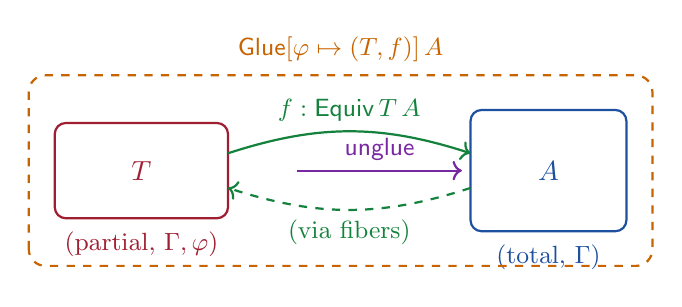
\begin{tikzpicture}[baseline={(0,0)}, scale=1.1]
  % A box
  \draw[thick, deepblue, rounded corners=4pt] (1.6,-0.7) rectangle (3.4,0.7);
  \node[deepblue] at (2.5, 0) {$A$};
  \node[deepblue, font=\small] at (2.5,-1.0) {(total, $\Gamma$)};

  % T box
  \draw[thick, deepred, rounded corners=4pt] (-3.2,-0.55) rectangle (-1.2,0.55);
  \node[deepred] at (-2.2,0) {$T$};
  \node[deepred, font=\small] at (-2.2,-0.85) {(partial, $\Gamma,\varphi$)};

  % Equiv arrow
  \draw[->, thick, deepgreen] (-1.2, 0.2) to[bend left=18]
    node[above, font=\small]{$f : \EquivT\,T\,A$} (1.6, 0.2);
  \draw[->, thick, deepgreen, dashed] (1.6,-0.2) to[bend left=18]
    node[below, font=\small]{(via fibers)} (-1.2,-0.2);

  % Glue type border
  \draw[thick, deeporange, rounded corners=6pt, dashed]
    (-3.5,-1.1) rectangle (3.7, 1.1);
  \node[deeporange, font=\small\bfseries] at (0.1, 1.4)
    {$\GlueT\sys{\varphi}{(T,f)}\,A$};

  % unglue arrow
  \draw[->, thick, deeppurple]
    (-0.4, 0) -- (1.5, 0) node[midway, above, font=\small]{$\unglueT$};
\end{tikzpicture}
\]

$\unglueT : \GlueT\sys{\varphi}{(T,f)}\,A \to A$ is the projection that
\emph{extends} $f$: it agrees with $f$ wherever $\varphi$ holds.

\subsection{Why \texttt{unglue} is the key map}

The theorem that $\unglueT$ is itself an equivalence is precisely the
univalence axiom. The intuition is:
\begin{itemize}
  \item $\unglueT$ is surjective: given $a : A$, use the equivalence $f$ on
        the face $\varphi$ to find the preimage $t : T$, then glue to get a
        total element of $\GlueT$.
  \item $\unglueT$ is injective: the $\eta$-rule $b = \glueT\sys{\varphi}{b}
        (\unglueT\,b)$ says every Glue element is fully determined by its
        $\unglueT$ projection.
\end{itemize}

%──────────────────────────────────────────────────────────────────────────────
\section{Composition for Glueing}
%──────────────────────────────────────────────────────────────────────────────

\subsection{Setup and goal}

Assume $\Gamma,\, i : \III \vdash B = \GlueT\sys{\varphi}{(T,f)}\,A$.
Given
\[
  \Gamma,\, \psi,\, i : \III \vdash b : B
  \qquad\text{and}\qquad
  \Gamma \vdash b_0 : B(\io)\sys{\psi}{b(\io)}
\]
we want to compute $\compT^i\, B\sys{\psi}{b}\, b_0 : B(\ii)\sys{\psi}{b(\ii)}$.

\subsection{The algorithm (CCHM \S6.2)}

Define the following auxiliary terms, with their contexts:

\medskip
\begin{center}
\renewcommand{\arraystretch}{1.5}
\begin{tabular}{@{}llll@{}}
\hline
\textbf{Name} & \textbf{Definition} & \textbf{Context} & \textbf{Type} \\
\hline
$a$ & $\unglueT\, b$ & $\Gamma,\psi,i:\III$
  & $A\sys{\varphi}{f\,b}$ \\
$a_0$ & $\unglueT\, b_0$ & $\Gamma$
  & $A(\io)\sys{\varphi(\io)}{f(\io)\,b_0,\,\psi}{a(\io)}$ \\
$\delta$ & $\forall i.\,\varphi$ & $\Gamma$
  & (the ``always-on'' part of $\varphi$) \\
$a'_1$ & $\compT^i\, A\sys{\psi}{a}\, a_0$ & $\Gamma$
  & $A(\ii)$ \\
$t'_1$ & $\compT^i\, T\sys{\psi}{b}\, b_0$ & $\Gamma,\delta$
  & $T(\ii)$ \\
$\omega$ & $\pres{i}\, f\sys{\psi}{b}\, b_0$ & $\Gamma,\delta$
  & path: $f(\ii)\,t'_1 \leadsto a'_1$ \\
$(t_1,\alpha)$ & $\equivT\, f(\ii)
  \sys{\delta}{(t'_1,\omega),\,\psi}{(b(\ii),\,\mathrm{refl})}\, a'_1$
  & $\Gamma,\varphi(\ii)$
  & $T(\ii)$ and correction path $\alpha$ \\
$a_1$ & $\compT^j\, A(\ii)
  \sys{\varphi(\ii)}{\alpha_j,\,\psi}{a(\ii)}\, a'_1$
  & $\Gamma$ & $A(\ii)$ \\
$b_1$ & $\glueT\sys{\varphi(\ii)}{t_1}\, a_1$ & $\Gamma$
  & $B(\ii)$ \quad \textbf{(result)} \\
\hline
\end{tabular}
\end{center}

\subsection{Step-by-step intuition}

\begin{enumerate}[label=\textbf{Step \arabic*.}]
  \item \textbf{Unglue to $A$.} Project the partial tube $b$ and base $b_0$
        to $A$ via $\unglueT$. Since $A$ is fibrant (supports composition),
        we can compose in $A$.

  \item \textbf{Compose in $A$.} Compute $a'_1$ — the ``naive'' $A$-level
        result at $\ii$.

  \item \textbf{Compose in $T$ (on $\delta = \forall i.\varphi$).} When
        $\varphi$ holds for all $i$, we also have a $T$-level computation
        $t'_1$.

  \item \textbf{Apply the equiv operation.} On the face $\varphi(\ii)$, use
        the equivalence $f(\ii)$ to find a $T$-element $t_1$ mapping (up to a
        path $\alpha$) to $a'_1$. The correction path $\alpha$ accounts for
        the discrepancy between the $A$-composition and the image of the
        $T$-composition.

  \item \textbf{Correct in $A$.} Compose along $\alpha$ to get the final
        $A$-element $a_1$ that is compatible with $t_1$.

  \item \textbf{Glue.} Wrap up as $\glueT\sys{\varphi(\ii)}{t_1}\, a_1$.
        This is well-typed because $a_1 : A(\ii)\sys{\varphi(\ii)}{f(\ii)\,t_1}$.
\end{enumerate}

\begin{remark}
  When $\varphi = \topF$ (so $B = T$ everywhere), the algorithm reduces to
  $\compT^i\, T\sys{\psi}{b}\, b_0$, as expected from the $\topF$-reduction.
\end{remark}

%──────────────────────────────────────────────────────────────────────────────
\section{Composition for the Universe}
%──────────────────────────────────────────────────────────────────────────────

\subsection{Constructing an equivalence from a line of types}

Given $\Gamma,\,i:\III \vdash E$ with $E(\io) = A$ and $E(\ii) = B$, define:
\begin{align*}
  f &= \lambda x : A.\; \transpT^i\, E\, x
    &&\text{(type $A \to B$)} \\
  g &= \lambda y : B.\; (\transpT^i\, E(i/1-i)\, y)(i/1-i)
    &&\text{(type $B \to A$)} \\
  u &= \lambda x : A.\; \fillT^i\, E\, []\, x
    &&\text{(context $i:\III$, type $A \to E$)} \\
  v &= \lambda y : B.\; (\fillT^i\, E(i/1-i)\, []\, y)(i/1-i)
    &&\text{(context $i:\III$, type $B \to E$)}
\end{align*}
satisfying $u(\io) = \mathrm{id}_A$, $u(\ii) = f$, $v(\io) = g$,
$v(\ii) = \mathrm{id}_B$.

One then proves $f$ is an equivalence by constructing contractible fibers
using nested fills and compositions (\S7.1 of CCHM), obtaining
$\eqop{i}\, E : \EquivT\, A\, B$.

\subsection{Composition for $\UU$}

\begin{equation}\label{eq:comp-U}
\boxed{
  \compT^i\, \UU\sys{\varphi}{E}\, A_0
  \;=\;
  \GlueT\bigl[\varphi \mapsto \bigl(E(\ii),\;\eqop{i}\,E(i/1-i)\bigr)\bigr]\, A_0
  \;:\; \UU
}
\end{equation}
To compose along a partial line of types $E$ over $\varphi$ from base $A_0$,
we construct the Glue type attaching $E(\ii)$ via the equivalence derived
from the line. The reversal $i/1-i$ gives an equivalence $E(\ii) \simeq A_0$.

%──────────────────────────────────────────────────────────────────────────────
\section{From Equivalence to Path}
%──────────────────────────────────────────────────────────────────────────────

\begin{example}[ua: Equiv to Path]\label{ex:ua}
  Given $\Gamma \vdash f : \EquivT\, A\, B$, define in context $\Gamma, i:\III$:
  \[
    E \;=\; \GlueT\bigl[(i=\io) \mapsto (A,f),\; (i=\ii) \mapsto (B,\mathrm{id}_B)\bigr]\, B
  \]
  where $\mathrm{id}_B = (\lambda x.\,x,\,\ldots) : \EquivT\, B\, B$.
  Then $E(\io) = A$ and $E(\ii) = B$ by $\topF$-reduction. So:
  \[
    \pt{ua}
    \;=\;
    \lambda A\,B.\;\lambda f : \EquivT\,A\,B.\;
    \langle i \rangle\,
    \GlueT\bigl[(i=\io) \mapsto (A,f),\;(i=\ii)\mapsto(B,\mathrm{id}_B)\bigr]\,B
    \;:\; (A\,B:\UU) \to \EquivT\,A\,B \to \PathT_\UU\,A\,B
  \]
\end{example}

%──────────────────────────────────────────────────────────────────────────────
\section{The Univalence Axiom as a Theorem}
%──────────────────────────────────────────────────────────────────────────────

\subsection{The main theorem}

\begin{theorem}[Theorem~9 of CCHM]\label{thm:unglue-equiv}
  Let $B = \GlueT\sys{\varphi}{(T,f)}\,A$.  The map
  $\unglueT : B \to A$
  is an equivalence.
\end{theorem}

\begin{proof}
  By Lemma~\ref{lem:equiv} (the equiv operation), it suffices to construct,
  given
  \[
    \Gamma,\,\psi \vdash b : B, \qquad
    \Gamma \vdash u : A, \qquad
    \Gamma,\,\psi \vdash \alpha : \PathT_A\, u\, (\unglueT\, b)
  \]
  a total lift:
  \[
    \tilde{b} : B\sys{\psi}{b}
    \qquad\text{and}\qquad
    \tilde{\alpha} : \PathT_A\, u\, (\unglueT\,\tilde{b})\sys{\psi}{\alpha}
  \]

  \medskip\noindent\textbf{Step 1: Lift on face $\varphi$.}
  On the combined face $\varphi \wedge \psi$ we have $b : T$ (since Glue
  elements are $T$-elements on $\varphi$) and
  $\alpha : \PathT_A\, u\, (f\,b)$.
  Applying Lemma~\ref{lem:equiv} to $f$ (which is an equivalence on
  $\varphi$):
  \[
    \Gamma,\,\varphi \vdash t : T\sys{\psi}{b}
    \qquad
    \Gamma,\,\varphi \vdash \beta : \PathT_A\, u\, (f\,t)\sys{\psi}{\alpha}
  \]

  \medskip\noindent\textbf{Step 2: Compose in $A$.}
  Define
  \[
    \tilde{a} = \compT^i\, A\sys{\varphi}{\beta_i,\,\psi}{\alpha_i}\, u \;:\; A
  \]
  using $\beta$ on $\varphi$ and $\alpha$ on $\psi$ as the partial tube.

  \medskip\noindent\textbf{Step 3: Construct the lift.}
  Set
  \[
    \tilde{b} = \glueT\sys{\varphi}{t}\,\tilde{a}
    \qquad\text{and}\qquad
    \tilde{\alpha} = \fillT^i\, A\sys{\varphi}{\beta_i,\,\psi}{\alpha_i}\, u
  \]
  Verification:
  \begin{itemize}
    \item $\tilde{b} : \GlueT\sys{\varphi}{(T,f)}\,A$ since $t : T$ on
          $\varphi$ and $\tilde{a} : A\sys{\varphi}{f\,t}$. \checkmark
    \item $\tilde{b}\big|_\psi = \glueT\sys{\varphi}{b}\,(\unglueT\,b) = b$
          by the $\eta$-rule. \checkmark
    \item $\unglueT\,\tilde{b} = \unglueT\,(\glueT\sys{\varphi}{t}\,\tilde{a})
          = \tilde{a}$ by the $\beta$-rule. \checkmark
    \item $\tilde{\alpha} : \PathT_A\, u\, \tilde{a}$ with
          $\tilde{\alpha}\big|_\psi = \alpha$ from the fill boundary. \checkmark
  \end{itemize}
  This provides the required lift, so $\unglueT$ is an equivalence.
\end{proof}

\subsection{Contractibility and the univalence axiom}

\begin{corollary}[Corollary~10 of CCHM]
  For any $A : \UU$, the type $(X : \UU) \times \EquivT\, X\, A$ is
  contractible.
\end{corollary}

\begin{proof}
  By Lemma~5 of CCHM, it suffices to show any partial element
  $\varphi \vdash (T, f) : (X:\UU)\times\EquivT\,X\,A$ is path-equal to the
  restriction of a total element. The map
  $\unglueT : \GlueT\sys{\varphi}{(T,f)}\,A \to A$ is an equivalence by
  Theorem~\ref{thm:unglue-equiv}. Since proofs of $\isEquivT\,X\,A\,f.1$ are
  path-equal (the type is a proposition), any partial element of
  $(X:\UU)\times\EquivT\,X\,A$ is path-equal to the restriction of the total
  element $(\GlueT\sys{\varphi}{(T,f)}\,A,\; \unglueT)$.
\end{proof}

\begin{corollary}[Univalence Axiom — Corollary~11 of CCHM]
  For any $A, B : \UU$, the canonical map
  \[
    \pt{idToEquiv} : \PathT_\UU\, A\, B \to \EquivT\, A\, B
  \]
  is an equivalence.
\end{corollary}

\begin{proof}
  Both $(X : \UU) \times \PathT_\UU\, A\, X$ and $(X : \UU) \times
  \EquivT\, A\, X$ are contractible (the former by singleton contractibility;
  the latter by the previous corollary). A map between contractible types is
  an equivalence; the result follows by applying this to the fibers at $B$.
  (See Theorem~4.7.7 of the HoTT book, or Appendix~B of CCHM for two
  alternative direct proofs.)
\end{proof}

\begin{remark}
  Univalence is \emph{not} an axiom in CCHM — it is a \emph{theorem} that
  follows from:
  \begin{enumerate}
    \item The $\GlueT$ type former with $\topF$-reduction, $\eta$, and $\beta$
          rules;
    \item The composition algorithm for $\GlueT$ (Section~6.2), making it
          fibrant;
    \item Composition for the universe $\UU$ (Section~7.1).
  \end{enumerate}
\end{remark}

%──────────────────────────────────────────────────────────────────────────────
\section{Summary}
%──────────────────────────────────────────────────────────────────────────────

\begin{center}
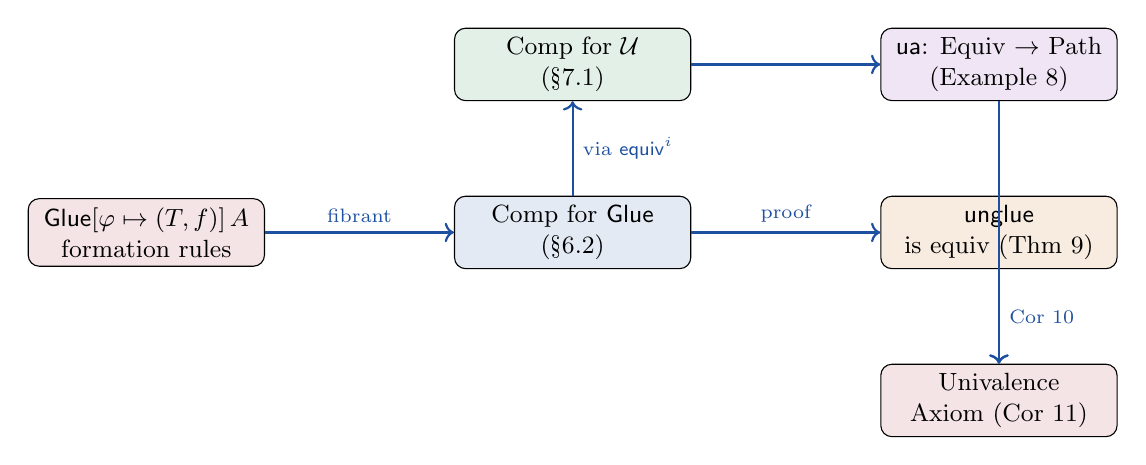
\begin{tikzpicture}[
  node distance=1.2cm and 2.4cm,
  box/.style={draw, rounded corners=4pt, fill=lightgray, align=center,
    minimum width=3.0cm, minimum height=0.75cm, font=\small},
  arr/.style={->, thick, deepblue},
]
  \node[box, fill=deepred!12]   (glue)  {$\GlueT\sys{\varphi}{(T,f)}\,A$\\formation rules};
  \node[box, right=of glue, fill=deepblue!12]  (compG) {Comp for $\GlueT$\\(§6.2)};
  \node[box, above=of compG, fill=deepgreen!12] (compU) {Comp for $\UU$\\(§7.1)};
  \node[box, right=of compG, fill=deeporange!12] (thm9) {$\unglueT$\\is equiv (Thm~9)};
  \node[box, above=of thm9, fill=deeppurple!12]  (ua)   {$\pt{ua}$: Equiv $\to$ Path\\(Example~8)};
  \node[box, below=of thm9, fill=deepred!12]    (univ) {Univalence\\Axiom (Cor~11)};

  \draw[arr] (glue)  -- (compG) node[midway,above,font=\scriptsize]{fibrant};
  \draw[arr] (compG) -- (compU) node[midway,right,font=\scriptsize]{via $\eqop{i}$};
  \draw[arr] (compG) -- (thm9)  node[midway,above,font=\scriptsize]{proof};
  \draw[arr] (compU) -- (ua)    node[midway,above,font=\scriptsize]{};
  \draw[arr] (thm9)  -- (univ)  node[midway,right,font=\scriptsize]{Cor~10};
  \draw[arr] (ua)    -- (univ)  node[midway,right,font=\scriptsize]{};
\end{tikzpicture}
\end{center}

\bigskip

\begin{center}
\renewcommand{\arraystretch}{1.3}
\begin{tabular}{@{}lll@{}}
\hline
\textbf{Concept} & \textbf{Role} & \textbf{Ref} \\
\hline
$\GlueT\sys{\varphi}{(T,f)}\,A$ & Glue $T$ onto $A$ via equiv $f$ on face $\varphi$ & §6.1 \\
$\glueT\sys{\varphi}{t}\,a$ & Introduce: pair partial $T$-term with $A$-term & §6.1 \\
$\unglueT\sys{\varphi}{f}\,b$ & Eliminate: extract $A$-component, extending $f$ & §6.1 \\
Comp for $\GlueT$ & Makes $\GlueT$ fibrant; 6-step algorithm & §6.2 \\
$\eqop{i}\,E$ & Equivalence from a line of types $E$ & §7.1 \\
$\compT^i\,\UU\sys{\varphi}{E}\,A_0$ & Composition for the universe & §7.1 \\
$\pt{ua}$ & Path from equivalence & §7, Ex.~8 \\
Thm~9 & $\unglueT$ is an equivalence & §7.2 \\
Cor~11 & Univalence axiom & §7.2 \\
\hline
\end{tabular}
\end{center}

\bigskip\noindent
The central insight: $\GlueT$ types are precisely the device that lets us
transport fibrancy across an equivalence boundary. Once we have $\GlueT$,
univalence falls out as a theorem.

\end{document}
